\documentclass{beamer}
\usetheme[...,logopath=./, logo=enes_blanco]{fibeamer}
\usepackage[utf8]{inputenc}
\usepackage[main=english]{babel}

%% These macros specify information about the presentation
\title{Detección de Digitos en las Manos} %% that will be typeset on the
\subtitle{Proyecto de Machine Learning} %% title page.
\author{Carlos Cortés}

%% These additional packages are used within the document:
\usepackage{ragged2e}  % `\justifying` text
\usepackage{booktabs}  % Tables
\usepackage{tabularx}
\usepackage{tikz}      % Diagrams

\usetikzlibrary{calc, shapes, backgrounds}

\usepackage{amsmath, amssymb}
\usepackage{url}       % `\url`s
\usepackage{listings}  % Code listings

\frenchspacing


\begin{document}
  \frame{\maketitle}

  \begin{darkframes}
    \section{Overview}
    \begin{frame}{Overview}
      \begin{tikzpicture}[overlay,remember picture]
        \node[anchor=south east,xshift=-30pt,yshift=35pt]
          at (current page.south east) {
            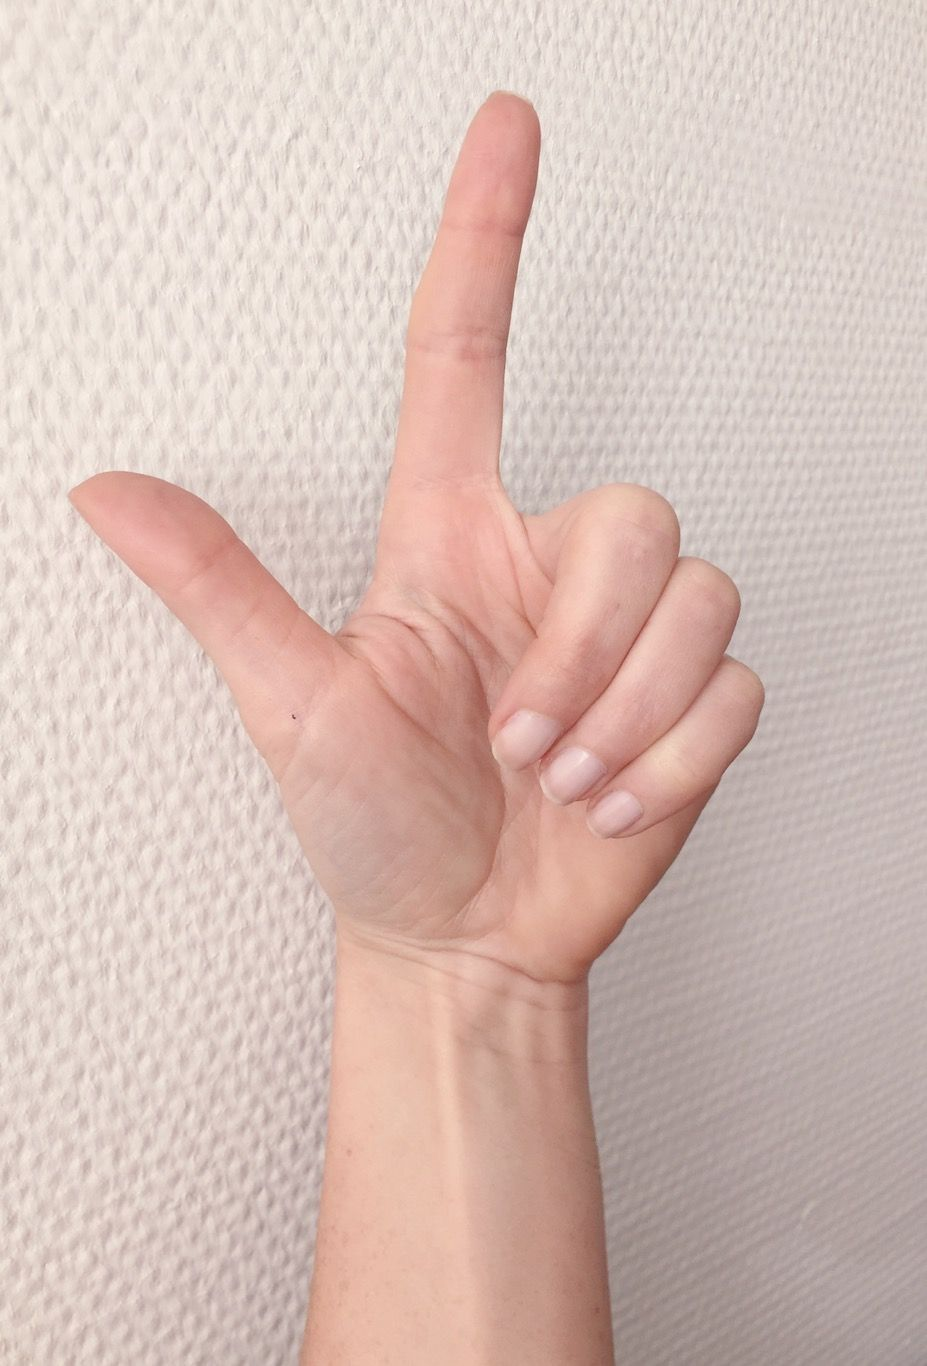
\includegraphics[width=35mm]{twoexample}
          };
      \end{tikzpicture}%
      \textbf{Objetivo: }Clasificar imágenes de manos\\
      haciendo dígitos de lenguaje de señas.\\ \bigskip \pause
      La idea surgió de querer reconocer el\\
      lenguaje de señas.\\
      Así que se intentó comenzar por reconocer\\
      únicamente los diez dígitos del\\
      lenguaje de señas.\\
      
      
    \end{frame}
    
    \section{Método}
    \begin{frame}{Método}
    Lo primordial es recordar que las imágenes son matrices.\\
    Podemos desdoblar la matriz en un gran vector para realizar machine learning con cada imagen como instancia.\\
    Se probó con dos métodos:
    \pause
    \begin{block}{K-NN}
        Es muy sencillo de realizar y da buenos resultados.\\
    \end{block}
    \pause
    \begin{block}{Regresión Logística.}
        Supuestamente da mejores resultados.
    \end{block}
    \end{frame}

    \section{Dataset}
    
    \begin{frame}{Preview}
        La base de datos de imágenes fue tomada del github de la referencia.\\
        Consta de 2062 imágenes etiquetadas del 0-9.\\
        Cada imagen es de 100x100 y en formato jpg (por lo que fue necesario convertirlas a escala de grises)~\cite{git}.
    \end{frame}
    \begin{frame}{Preview}
        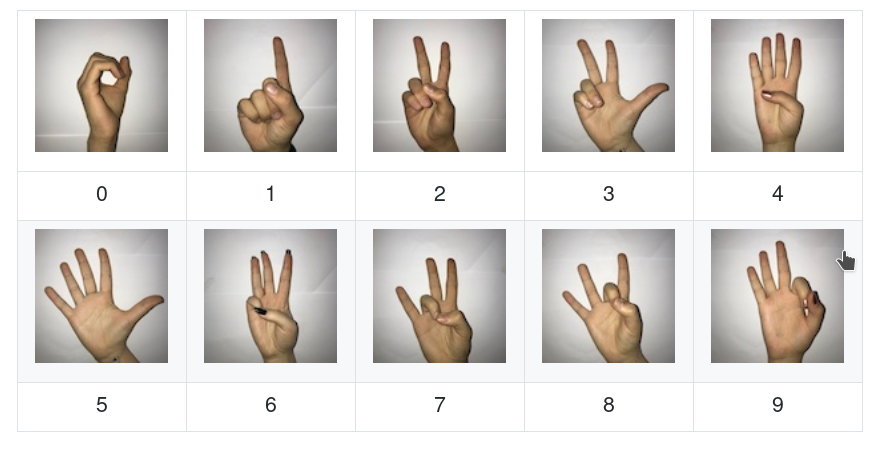
\includegraphics[scale=0.46]{dataset_preview}
    \end{frame}
    
    \section{Implementación}
    \begin{frame}{Dependencias}
        \begin{itemize}
         \item \emph{Mlpack}.\\
         Biblioteca principal para métodos de Machine Learning.\pause
         \item \emph{Armadillo}.\\
         Biblioteca para matrices que Mlpack utiliza.\pause
         \item \emph{OpenCV}.\\
         Biblioteca que utilizo para manipular imágenes y convertirlas en vectores.
        \end{itemize}

    \end{frame}
    
    \section{Código}
    \begin{frame}{Código}{Visita Rápida}
     \begin{center}
      Kdevelop.jpg
     \end{center}

    \end{frame}

    \section{Mejor Puntaje}
    \begin{frame}{Mejor Puntaje}
Partiendo el Dataset en 1856 de entramiento y 206 de prueba.\\
Con k = 10 vecinos más cercanos.\\

\begin{block}{K-NN}
        154 casos correctos.\\
        Porcentaje = $74.75\%$.\\
        Entre ($68.85\%$ , $80.65\%$) al $95\%$ de confianza.
    \end{block}
    \pause
    \begin{block}{Regresión Logística.}
        25 casos correctos.\\
        Porcentaje = $12.13\%$.\\
        Entre ($7.69\%$ , $16.57\%$) al $95\%$ de confianza.
    \end{block}
    \end{frame}
    
    \section{Better, Stronger}

\begin{frame}{Better, Stronger}
    Lo siguiente a hacer para mejorar/perfeccionar el proyecto:\pause
    \begin{itemize}
     \item Incluir una cámara para realizar clasificación en tiempo real.\pause
     \item Intentar aplicar PCA o alguna otra técnica que pudiera ayudar a aumentar el poder predictivo.\pause
     \item Seguir intento variantes de regresión logística (básicamente intentar redes neuronales).
    \end{itemize}

\end{frame}



    \begin{frame}[label=bibliography]{Bibliography}
      \begin{thebibliography}{9}
        \bibitem{git}
            ardamavi.
            Sign-Language-Digits-Dataset.
            2018.
            Recuperado de \url{https://github.com/ardamavi/Sign-Language-Digits-Dataset}
      \end{thebibliography}
    \end{frame}

  \end{darkframes}
\end{document}
